\documentclass{beamer}
\usetheme{metropolis}
\usepackage[utf8]{inputenc}
\usepackage[estonian]{babel}
%\usepackage[english=british]{csquotes}
\usepackage[autostyle=false]{csquotes}
\usepackage{multirow}

\usepackage[normalem]{ulem}

\title{IDU1321. Ettevõtte äriarhitektuur}
\subtitle{Seitsmes loeng}
%\date{10.09.2017}
\author{Andres Kütt}
\institute{Arhitekt}


\begin{document}

\begin{frame}
\titlepage
\end{frame}

%\begin{frame}[standout]
%Eksami kuupäev?
%\end{frame}

\begin{frame}[standout]
Küsimusi kodutöö kohta?
\end{frame}


\begin{frame}{Kus me oleme?}
	\begin{center}
		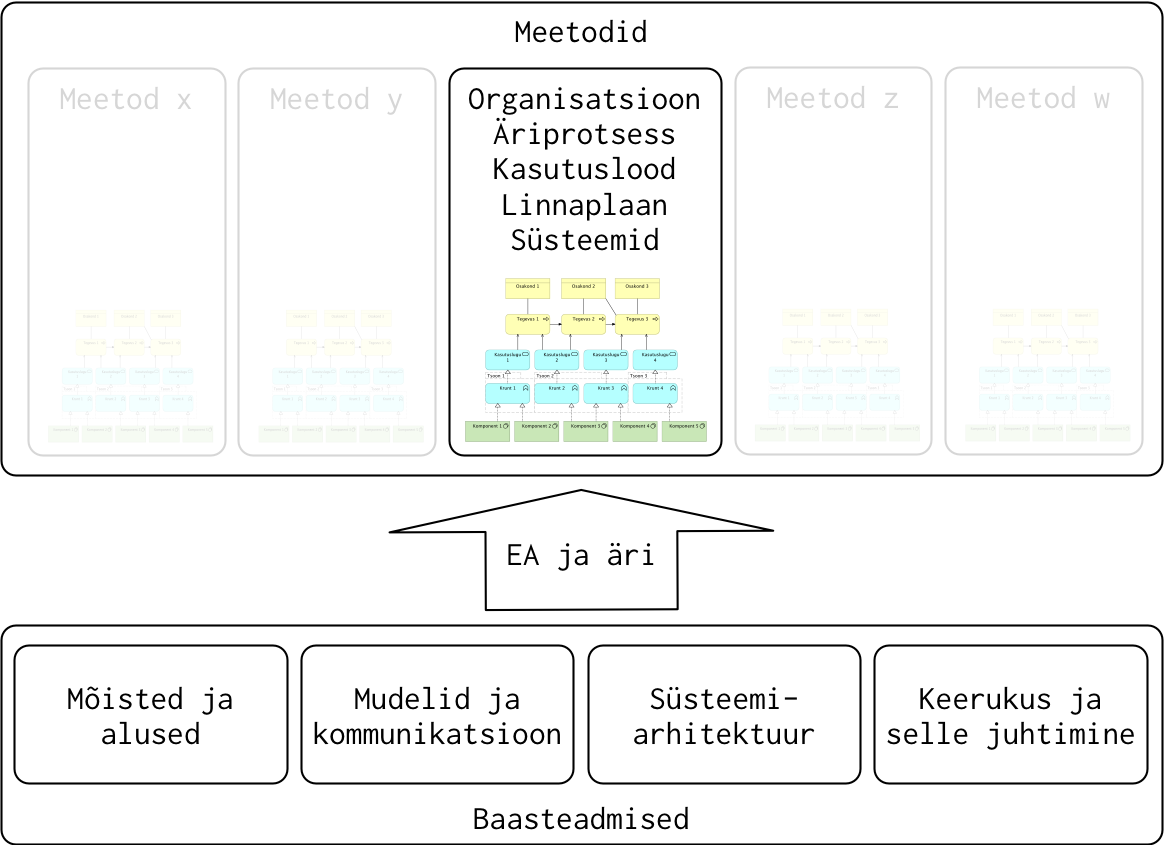
\includegraphics[width=.8\textwidth]{aine_struktuur}
	\end{center}
\end{frame}

\section{Süsteemiarhitektuur}
\begin{frame}[fragile]
	\begin{center}
		\LARGE{\textbf{Meil on vaja printsiipe, meetodeid ja vahendeid arhitektuuriga tegelemiseks}}
		\\[4cm]
		\small{Võimaldab tervikvaadet (ettevõte!), ennustab emergentsi, toetab väärtuse teket ja on praktiliselt kasulik}
	\end{center}
\end{frame}

\begin{frame}{Arhitektuuri definitsioon}
	\blockquote{The embodiment of concept, and the allocation of physical/informational function (process) to elements of form (objects) and definition of structural interfaces among the objects}

\cite{sysengineering}

\end{frame}

\begin{frame}{Definitsioonist}
	\begin{itemize}
		\item Mida ja kuidas tehakse moodustab lahutamatu terviku
		\item Jutt on nii vormi kui funktsiooni struktuurist
		\item Olulisel kohal on seosed tükkide vahel
	\end{itemize}
	\begin{center}
		Kuidas see kõik sobitub meie kodutööga?
	\end{center}
\end{frame}

\begin{frame}{Organisatsiooni arhitektuur}
	\begin{center}
		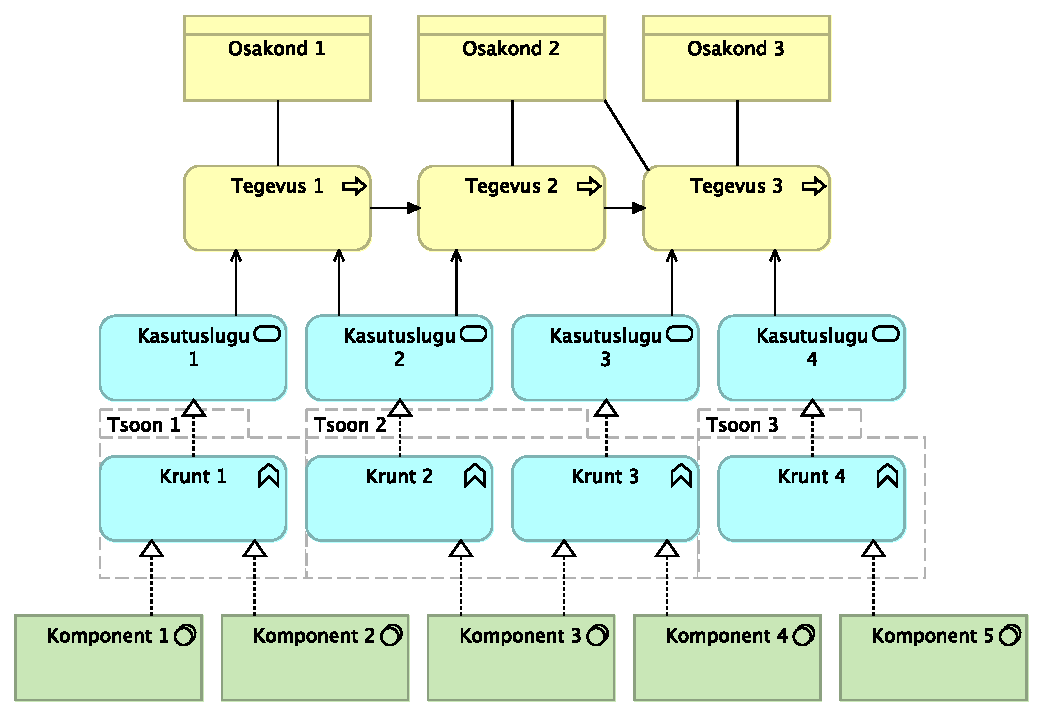
\includegraphics[width=\textwidth]{kihid}
	\end{center}
\end{frame}

\begin{frame}{Süsteemi arhitektuuri aspektid}
	\begin{center}
		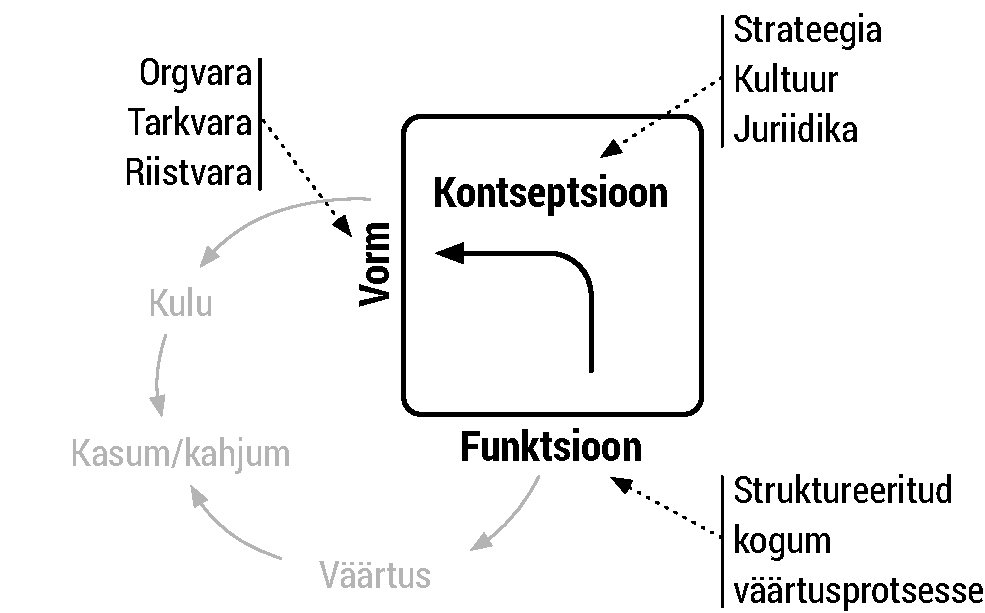
\includegraphics[width=.8\textwidth]{orgstruktuur}
	\end{center}
\end{frame}

\begin{frame}{Vorm, funktsioon, kontseptsioon}
	\begin{description}
		\item[Vorm] on miski, mis on. Ajas stabiilne
		\item[Funktsioon] on miski, mida vorm teeb. Sünnib ajas
		\item[Kontseptsioon] on viis, kuidas funktsiooni täidetakse. Peamised mõttemallid
	\end{description}
\end{frame}

\begin{frame}{Vorm ja funktsioon}
\begin{table}
\small
\begin{tabular}{|l|l|l|l|}
\hline
\multicolumn{1}{|c|}{\multirow{2}{*}{\textbf{Süsteem}}} & \multicolumn{1}{c|}{\multirow{2}{*}{\textbf{Vorm}}} & \multicolumn{2}{c|}{\textbf{Funktsioon}} \\ \cline{3-4} 
\multicolumn{1}{|c|}{} & \multicolumn{1}{c|}{} & \multicolumn{1}{c|}{\textbf{Protsess}} & \multicolumn{1}{c|}{\textbf{Operand}} \\ \hline
Võimendi & Võimendi elektroskeem & Võimendab & sisendsignaali \\ \hline
Meeskond & Meeskonna liikmed & Loob & disaini \\ \hline
Inimese vereringe & Vereringe & Varustab & hapnikuga \\ \hline
Sulepea & Tint, sulg, sulepea & Teeb & joont paberile \\ \hline
\end{tabular}\end{table}
\end{frame}

\section{Neli sammu}

\begin{frame}{Süsteemist mõtlemise neli sammu}
	Meie kodutöö on üks võimalusi neid samme tarkvara puhul läbi viia
	
		\begin{enumerate}
			\item Identify the the system, its form and function
			\item Identify the entities of the system, their form and function, the system boundary and context
			\item Identify relationships among the entities
			\item Predict emergence
		\end{enumerate}
\cite{crawley2015system}
\end{frame}


\begin{frame}{Millest süsteem koosneb?}
	Algoritm teise sammu läbimiseks
	
			\begin{itemize}
				\item Define the initial decomposition
				\item Identify the potential entities (holistic)
				\item Include the important entities of the system (focus)
				\item Create or recognise abstractions of the entities
				\item Define the boundary, separate the system from its context
			\end{itemize}
\cite{crawley2015system}
\end{frame}


\section{Harjutus}

\begin{frame}
	Harjutame süsteemide vormi, funktsiooni ja kontseptsiooni tuvastamist
	\begin{itemize}
		\item \enquote{Nelja sammu} ei pea järgima aga nad võivad abiks olla
		\item Iga süsteemi kohta
		\begin{itemize}
			\item Määratlege vorm
			\item Määratlege funktsioon skeemi \enquote{protsess + operand} kaudu
			\item Peamised kontseptsiooni elemendid
		\end{itemize}
		\item Laualambi näide:
		\begin{description}
			\item[Vorm] Alus, vars, juhtmed, lüliti, LED pirn
			\item[Funktsioon] Anda lauale valgust
			\item[Kontseptsioon] Täidan funktsiooni pooljuhist alalisvoolu läbi laskmise teel
		\end{description}
	\end{itemize}
\end{frame}

\begin{frame}{Harjutus}

\begin{itemize}
	\item Uurige süsteeme
	\begin{enumerate}
		\item Pastakas
		\item Skype
		\item Mobiilivõrk
		\item Õppejõud
		\item TTÜ
		\item ERP
\end{enumerate}
	\item Tegutsege paarides
	\begin{itemize}
		\item 18 minutit tööd süsteemide kallal
		\item 12 minutit esitlete oma tulemust kõrvalpaarile ja kuulate nende oma
	\end{itemize}
\end{itemize}
\end{frame}


\begin{frame}{Harjutuse kokkuvõte}
	\begin{itemize}
		\item Kuidas erinevad mobiilivõrk ja Skype?
		\item Kuidas õnnestus funktsiooni vormist eristamine?
		\item Millest koosneb õppejõud?
	\end{itemize}
\end{frame}


\begin{frame}{Kordame}
	\begin{itemize}
		\item Süsteemiarhitektuuri eesmärgiks on anda arhitekti toimetamisele teadmistepõhine alus
		\item Arhitekt tegeleb asjade osade, nende funktsiooni ning seostega
		\item Eksisteerib efektiivne meetod süsteemi struktuuri kirjeldamiseks
	\end{itemize}
\end{frame}

\begin{frame}{Järgmine kord}
\begin{center}
Keerulised asjad ja miks on neist kasulik mõelda
\end{center}
\end{frame}

\begin{frame}{Bibliography}
	\bibliographystyle{plainnat}
	\bibliography{idu1321}
\end{frame}

\begin{frame}[standout]
Küsimusi?
\end{frame}

\end{document}
